% Adjust these for the path of the theme and its graphics, relative to this file
%\usepackage{beamerthemeFalmouthGamesAcademy}
\usepackage{../../beamerthemeFalmouthGamesAcademy}
\usepackage{multimedia}
\graphicspath{ {../../} }

% Default language for code listings
\lstset{language=C++,
        morekeywords={each,in,nullptr}
}

% From http://blog.virtualglobebook.com/2011/02/syntax-highlighting-c-and-glsl-source.html

\lstdefinelanguage{GLSL}
{
sensitive=true,
morekeywords=[1]{
attribute, const, uniform, varying,
layout, centroid, flat, smooth,
noperspective, break, continue, do,
for, while, switch, case, default, if,
else, in, out, inout, float, int, void,
bool, true, false, invariant, discard,
return, mat2, mat3, mat4, mat2x2, mat2x3,
mat2x4, mat3x2, mat3x3, mat3x4, mat4x2,
mat4x3, mat4x4, vec2, vec3, vec4, ivec2,
ivec3, ivec4, bvec2, bvec3, bvec4, uint,
uvec2, uvec3, uvec4, lowp, mediump, highp,
precision, sampler1D, sampler2D, sampler3D,
samplerCube, sampler1DShadow,
sampler2DShadow, samplerCubeShadow,
sampler1DArray, sampler2DArray,
sampler1DArrayShadow, sampler2DArrayShadow,
isampler1D, isampler2D, isampler3D,
isamplerCube, isampler1DArray,
isampler2DArray, usampler1D, usampler2D,
usampler3D, usamplerCube, usampler1DArray,
usampler2DArray, sampler2DRect,
sampler2DRectShadow, isampler2DRect,
usampler2DRect, samplerBuffer,
isamplerBuffer, usamplerBuffer, sampler2DMS,
isampler2DMS, usampler2DMS,
sampler2DMSArray, isampler2DMSArray,
usampler2DMSArray, struct},
morekeywords=[2]{
radians,degrees,sin,cos,tan,asin,acos,atan,
atan,sinh,cosh,tanh,asinh,acosh,atanh,pow,
exp,log,exp2,log2,sqrt,inversesqrt,abs,sign,
floor,trunc,round,roundEven,ceil,fract,mod,modf,
min,max,clamp,mix,step,smoothstep,isnan,isinf,
floatBitsToInt,floatBitsToUint,intBitsToFloat,
uintBitsToFloat,length,distance,dot,cross,
normalize,faceforward,reflect,refract,
matrixCompMult,outerProduct,transpose,
determinant,inverse,lessThan,lessThanEqual,
greaterThan,greaterThanEqual,equal,notEqual,
any,all,not,textureSize,texture,textureProj,
textureLod,textureOffset,texelFetch,
texelFetchOffset,textureProjOffset,
textureLodOffset,textureProjLod,
textureProjLodOffset,textureGrad,
textureGradOffset,textureProjGrad,
textureProjGradOffset,texture1D,texture1DProj,
texture1DProjLod,texture2D,texture2DProj,
texture2DLod,texture2DProjLod,texture3D,
texture3DProj,texture3DLod,texture3DProjLod,
textureCube,textureCubeLod,shadow1D,shadow2D,
shadow1DProj,shadow2DProj,shadow1DLod,
shadow2DLod,shadow1DProjLod,shadow2DProjLod,
dFdx,dFdy,fwidth,noise1,noise2,noise3,noise4,
EmitVertex,EndPrimitive},
morekeywords=[3]{
gl_VertexID,gl_InstanceID,gl_Position,
gl_PointSize,gl_ClipDistance,gl_PerVertex,
gl_Layer,gl_ClipVertex,gl_FragCoord,
gl_FrontFacing,gl_ClipDistance,gl_FragColor,
gl_FragData,gl_MaxDrawBuffers,gl_FragDepth,
gl_PointCoord,gl_PrimitiveID,
gl_MaxVertexAttribs,gl_MaxVertexUniformComponents,
gl_MaxVaryingFloats,gl_MaxVaryingComponents,
gl_MaxVertexOutputComponents,
gl_MaxGeometryInputComponents,
gl_MaxGeometryOutputComponents,
gl_MaxFragmentInputComponents,
gl_MaxVertexTextureImageUnits,
gl_MaxCombinedTextureImageUnits,
gl_MaxTextureImageUnits,
gl_MaxFragmentUniformComponents,
gl_MaxDrawBuffers,gl_MaxClipDistances,
gl_MaxGeometryTextureImageUnits,
gl_MaxGeometryOutputVertices,
gl_MaxGeometryOutputVertices,
gl_MaxGeometryTotalOutputComponents,
gl_MaxGeometryUniformComponents,
gl_MaxGeometryVaryingComponents,gl_DepthRange},
morecomment=[l]{//},
morecomment=[s]{/*}{*/},
morecomment=[l][keywordstyle4]{\#},
}


% For strikethrough effect
\usepackage[normalem]{ulem}
\usepackage{wasysym}

\usepackage{pdfpages}

% http://www.texample.net/tikz/examples/state-machine/
\usetikzlibrary{arrows,automata}

\newcommand{\modulecode}{COMP260}\newcommand{\moduletitle}{Distributed Systems}\newcommand{\sessionnumber}{5}

\begin{document}
\title{\sessionnumber: Vertices, Transforms \& Projections}
\subtitle{\modulecode: \moduletitle}

\frame{\titlepage} 

\begin{frame}{Learning outcomes}
	By the end of this week, you should be able to:
	\begin{itemize}
		\item \textbf{Recall} alternative ways to represent mesh vertices in memory.
		\item \textbf{Apply} basic transforms using the GLM library.
		\item \textbf{Explain} the constituents of the model-view-projection matrix and how it can be used to create a first-person camera controller.
	\end{itemize}
\end{frame}

\begin{frame}{Agenda}
	\begin{itemize}
		\pause\item Lecture (async):
		\begin{itemize}
			\item \textbf{Compare} different ways to store vertex data in memory.
			\item \textbf{Review} the transforms required to display 3D objects on a 2D screen.
		\end{itemize}
		\pause\item Workshop (sync):
		\begin{itemize}
			\item \textbf{Adapt} our basic triangle implementation to draw meshes with multiple triangles efficiently.
			\item \textbf{Experiment} with creating transforms using GLM and using them to move objects and the camera.
		\end{itemize}
	\end{itemize}
\end{frame}

\part{Vertices}
\frame{\partpage}

\begin{frame}{Interleaved Vertices}
	\begin{itemize}
		\pause\item Up until this point we have been storing vertex positions as floats
		\pause\item If we need a vertex to have colours, we can store these in a separate Vertex Buffer
		\pause\item Or we can create a \textbf{C structure} which represents a Vertex, which has member variables which represent positions, colours, normals etc
		\pause\item This is known as Interleaved Vertices and in \pause\textbf{MOST} cases is more efficient
	\end{itemize}
\end{frame}

\begin{frame}[fragile]{Vertex Structure 1}
	\begin{lstlisting}
		struct Vertex
		{
			float x,y,z;
		};
		
		Vertex v[]={{-0.5f,-0.5f,0.0f},
					{0.5f,-0.5f,0.0f},
					{0.0f,0.5f,0.0f}};
					 
	\end{lstlisting}
\end{frame}

\begin{frame}[fragile]{Vertex Structure 2}
	\begin{lstlisting}
		struct Vertex
		{
			float x,y,z;
			float r,g,b,a;
		};
		
		Vertex v[]={{-0.5f,-0.5f,0.0f,1.0f,0.0f,0.0f,1.0f},
					{0.5f,-0.5f,0.0f,0.0f,1.0f,0.0f,1.0f},
					{0.0f,0.5f,0.0f,0.0f,0.0f,1.0f,1.0f}};
	\end{lstlisting}
\end{frame}

\begin{frame}{Changes to the Vertex Buffer}
	\begin{itemize}
		\pause\item There will be a slight change to our vertex buffer
		\pause\item We have to take into account the size of the Vertex structure and the number of vertices in the buffer
	\end{itemize}
\end{frame}

\begin{frame}[fragile]{Vertex Buffer Changes - Old version}
	\begin{lstlisting}
		glBufferData(GL_ARRAY_BUFFER, sizeof(g_vertex_buffer_data), g_vertex_buffer_data, GL_STATIC_DRAW);
	\end{lstlisting}
\end{frame}

\begin{frame}[fragile]{Vertex Buffer Changes - new version}
	\begin{lstlisting}
		glBufferData(GL_ARRAY_BUFFER, 3* sizeof(Vertex), v, GL_STATIC_DRAW);
	\end{lstlisting}
\end{frame}

\begin{frame}{Changes to the Vertex Array}
	\begin{itemize}
		\pause\item Since the layout of the vertices have changed in memory, we need to update the Vertex Array Object to reflect this
		\pause\item Remember that the VAO describes the format of the vertices to the pipeline and enables the binding of vertex data to attributes in the shader 
	\end{itemize}
\end{frame}

\begin{frame}[fragile]{Vertex Array Object - Old version}
\begin{lstlisting}
	glEnableVertexAttribArray(0);
	glVertexAttribPointer(0,3,GL_FLOAT,GL_FALSE,0,(void*)0);
\end{lstlisting}
\end{frame}

\begin{frame}[fragile]{Vertex Array Object - New version}
\begin{lstlisting}
	glEnableVertexAttribArray(0);
	glVertexAttribPointer(0,3,GL_FLOAT,GL_FALSE,sizeof(Vertex),(void*)0);
	
	glEnableVertexAttribArray(1);
	glVertexAttribPointer(1,4,GL_FLOAT,GL_FALSE,sizeof(Vertex),(void*)(3*sizeof(float)));
\end{lstlisting}
\end{frame}

\begin{frame}{Memory and Vertex Array Object 1}
		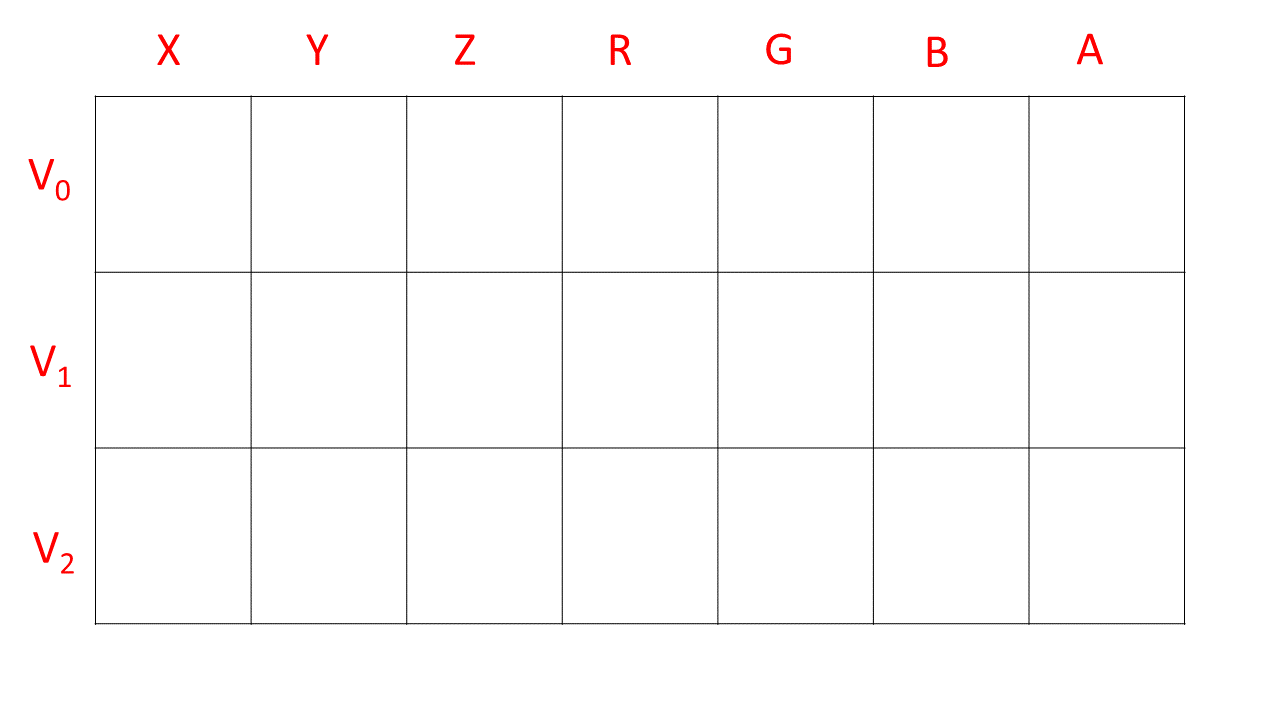
\includegraphics[height=0.8\textheight]{MemoryLayoutStarter}	
\end{frame}

\begin{frame}{Memory and Vertex Array Object 2}
	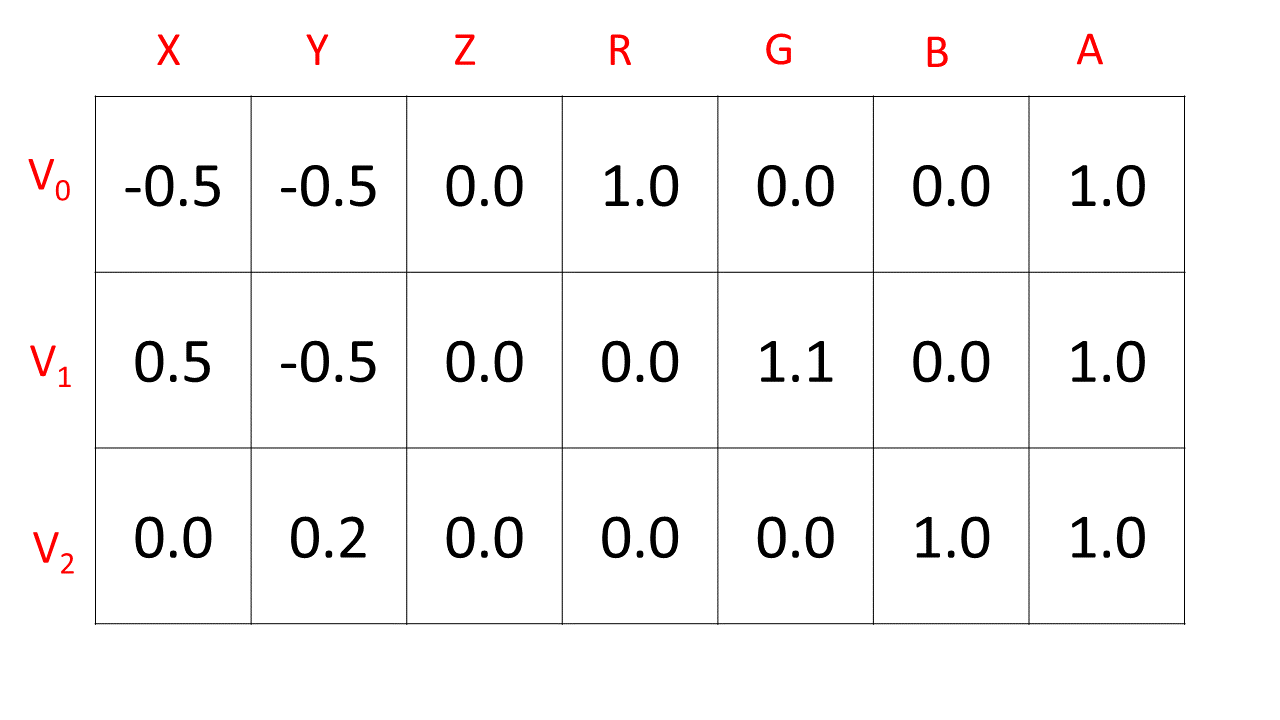
\includegraphics[height=0.8\textheight]{MemoryLayoutValues}	
\end{frame}

\begin{frame}{Memory and Vertex Array Object 3 - Stride}
	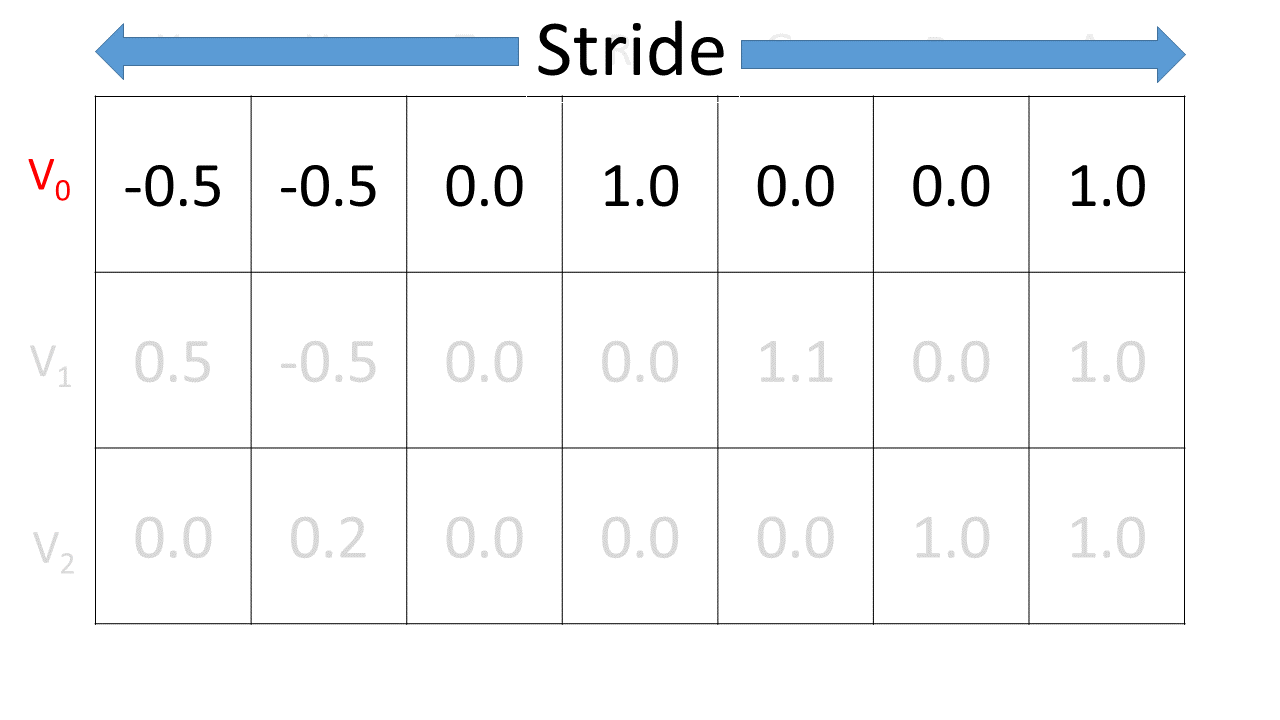
\includegraphics[height=0.8\textheight]{MemoryLayoutStride}	
\end{frame}

\begin{frame}{Memory and Vertex Array Object 3 - Offset}
	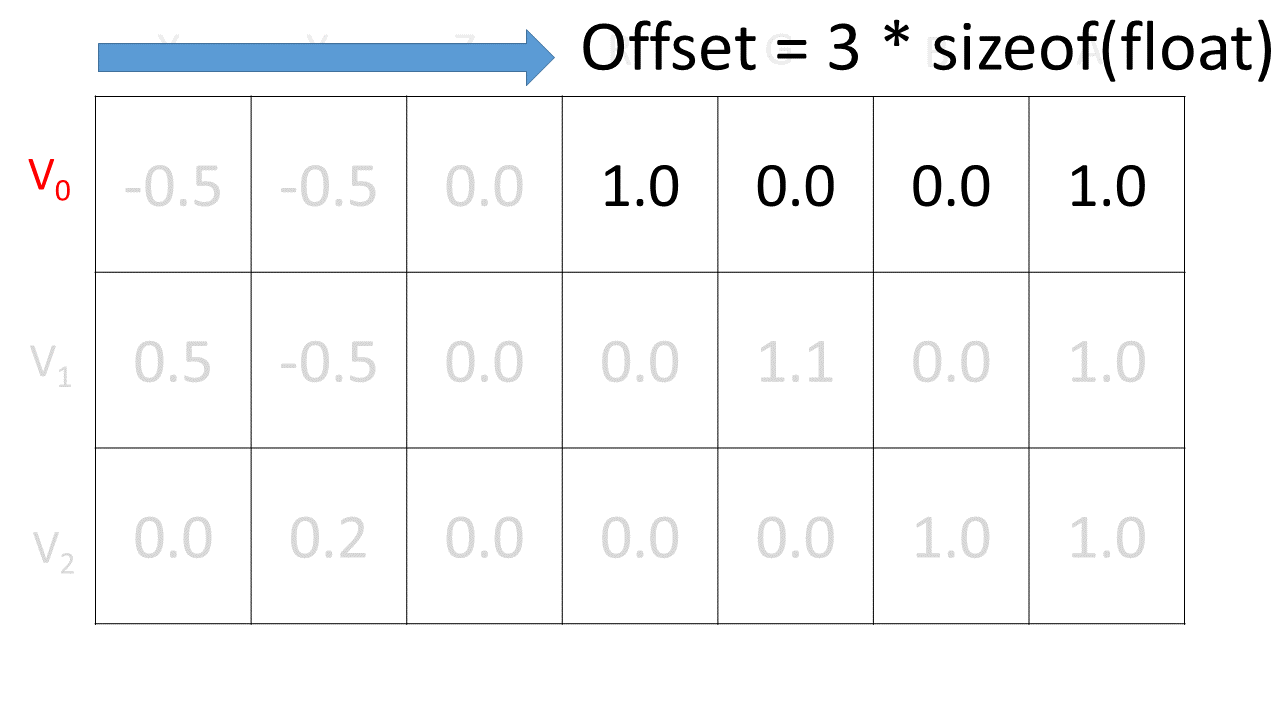
\includegraphics[height=0.8\textheight]{MemoryLayoutOffset}	
\end{frame}
\part{Model, View, Projection}
\frame{\partpage}

\begin{frame}{Model, View, Projection}
	\pause Drawing a 3D object on screen generally involves \textbf{three} transformations:
	\begin{itemize}
		\pause\item \textbf{Model}: translate, rotate and scale the object into its place in the scene
		\pause\item \textbf{View}: translate and rotate the scene to put the observer at the origin
		\pause\item \textbf{Projection}: convert points in 3D space to points on the 2D screen
	\end{itemize}
	\pause The \textbf{model-view-projection (MVP) matrix}:
		$$ M_{MVP} = M_{\text{projection}} \times M_{\text{view}} \times M_{\text{model}} $$
	(remember, multiplication goes in reverse order)
\end{frame}

\begin{frame}{The model matrix}
	\pause Exactly what we've been doing so far today...
\end{frame}

\begin{frame}[fragile]{The view matrix}
	\pause Need to translate and rotate the scene so that the ``camera'' is at $(0,0,0)$ and looking in the negative $z$ direction
	\pause\begin{lstlisting}
glm::mat4 view = glm::lookAt(
  glm::vec3(2, 0, 2),    // eye
  glm::vec3(0, 0, 0),    // centre
  glm::vec3 up(0, 1, 0)  // up
);
	\end{lstlisting}
	\begin{itemize}
		\pause\item \lstinline{eye} is the position of the camera
		\pause\item \lstinline{centre} is a point for the camera to look at
		\pause\item \lstinline{up} is which direction is ``up'' for the camera (usually the positive $y$-axis)
	\end{itemize}
\end{frame}

\begin{frame}{Types of projection}
	\pause\begin{center}
		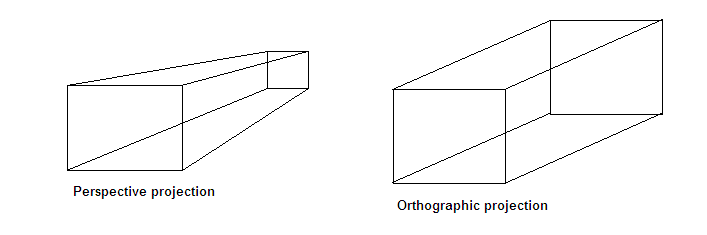
\includegraphics[width=\textwidth]{orthographic_perspective}
	\end{center}
	\begin{itemize}
		\pause\item Generally use \textbf{perspective} for 3D graphics
		\pause\item \textbf{Orthographic} is useful for 2D or pseudo-2D graphics (e.g.\ isometric perspective)
	\end{itemize}
\end{frame}

\begin{frame}[fragile]{The projection matrix}
	\pause\begin{lstlisting}
glm::mat4 projection = glm::perspective(
	glm::radians(45.0f), // field of view
	4.0f / 3.0f,         // aspect ratio
	0.1f,                // near clip plane
	100.0f               // far clip plane
);
	\end{lstlisting}
	\begin{itemize}
		\pause\item \textbf{Field of view (FOV)}: how ``wide'' or ``narrow'' the view is
		\pause\item \textbf{Aspect ratio}: should be \lstinline{screenWidth / screenHeight}
		\pause\item \textbf{Near and far clip planes}: fragments that fall outside this range of distances from the camera are not drawn
	\end{itemize}
	\pause Also available: \lstinline{glm::ortho} for orthographic projection
\end{frame}

\begin{frame}{The view frustum}
	\pause\begin{center}
		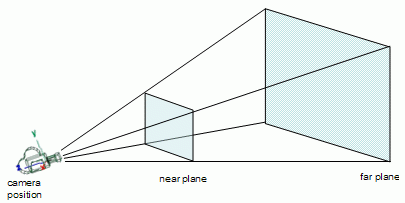
\includegraphics[width=0.8\textwidth]{frustum}
	\end{center}
	\begin{itemize}
		\pause\item Defined by the \textbf{near and far clipping planes} and the \textbf{edges of the screen}
		\pause\item \textbf{Nothing outside} the view frustum is visible
	\end{itemize}
\end{frame}

\begin{frame}[fragile]{Putting it together}
	\pause\begin{lstlisting}
glm::mat4 mvp = projection * view * modelTransform;
glUniformMatrix4fv(mvpLocation, 1, GL_FALSE, glm::value_ptr(mvp));
	\end{lstlisting}
	\pause And in the vertex shader, simply multiply the vertex position (in homogeneous coordinates) by the MVP matrix:
	\pause\begin{lstlisting}[language=GLSL]
uniform mat4 mvp;

void main()
{
  gl_Position = mvp * vec4(vertexPos, 1.0);
}
	\end{lstlisting}
\end{frame}

\part{First person camera control}
\frame{\partpage}

\begin{frame}{The plan}
	\begin{itemize}
		\pause\item Represent the player's \textbf{position} by a 3D vector
		\pause\item Represent the player's \textbf{orientation} by Euler angles
		\pause\item Mouse events change these angles
		\pause\item View matrix is calculated using position and orientation
		\pause\item To move forwards, use the Euler angles to find the ``forward'' vector,
			and offset the position by this vector
	\end{itemize}
\end{frame}

\begin{frame}{Keyboard and mouse in SDL}
	\pause Use \textbf{relative mouse mode}
	\begin{itemize}
		\pause\item Hides the mouse pointer
		\pause\item Prevents the mouse pointer from hitting the edge of the screen
		\pause\item Gives us the distance the mouse has moved since last frame, rather than its current position
	\end{itemize}
	\pause Use \lstinline{SDL_GetKeyboardState} instead of handling individual keyboard events
	\begin{itemize}
		\pause\item Allows us to check on every frame whether the key is held down
		\pause\item Otherwise, the player will move jerkily according to the key repeat rate
	\end{itemize}
\end{frame}

\begin{frame}{Vector addition}
	\pause
	\begin{center}
		\colorbox{white}{
			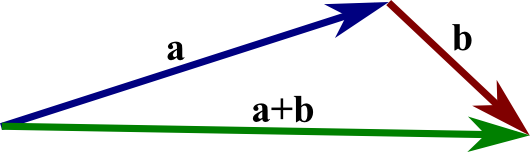
\includegraphics[width=0.5\textwidth]{vector_addition}
		}
	\end{center}
	\begin{itemize}
		\pause\item E.g.\ if $a$ is current position, and
		\pause\item $b$ is the distance and direction we want to move, then
		\pause\item $a + b$ is the new position
	\end{itemize}
\end{frame}

\begin{frame}{Addition in homogeneous coordinates}
	\begin{itemize}
		\pause\item Recall: homogeneous coordinates have an extra $w$ component, i.e.\ $(x,y,z,w)$
		\pause\item $w=1$ for positions, $w=0$ for offsets
	\end{itemize}
	\begin{tabular}{rclclc}
		\pause offset & + & offset & = & offset & $w = 0 + 0 = 0$ \\
		\pause position & + & offset & = & position & $w = 1 + 0 = 1$ \\
		\pause position & + & position & = & ??? & $w = 1 + 1 = 2$
	\end{tabular}
\end{frame}

\begin{frame}{Unit vectors}
	\begin{itemize}
		\pause\item A \textbf{unit vector} is a vector of length 1
		\pause\item I.e.\ $\sqrt{x^2 + y^2 + z^2} = 1$ (Pythagoras)
		\pause\item Useful to represent \textbf{direction}
		\pause\item Multiplying a vector of length $a$ by a number $b$ gives a vector of length $a \times b$,
			parallel to the original vector
		\pause\item So multiplying a unit vector by $b$ gives a vector of length $b$,
			parallel to the unit vector		
	\end{itemize}
\end{frame}

\begin{frame}{Representing look direction}
	\begin{columns}
		\pause
		\begin{column}{0.48\textwidth}
			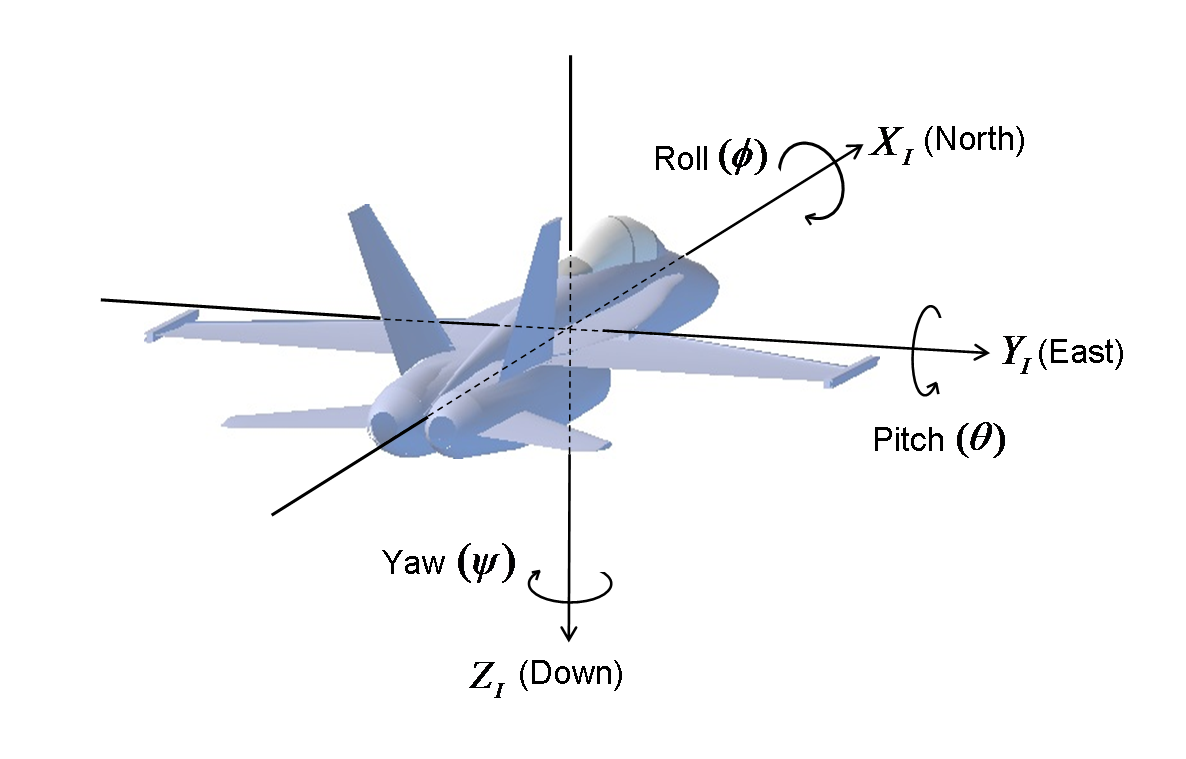
\includegraphics[width=\textwidth]{../03/euler_aeroplane}
		\end{column}
		\begin{column}{0.48\textwidth}
			\begin{itemize}
				\pause\item Euler angles
				\pause\item Don't need roll, just pitch and yaw
				\pause\item (Not using roll eliminates the gimbal lock problem)
				\pause\item Forward vector and look vector can be obtained by appropriate rotation of a unit vector
			\end{itemize}
		\end{column}
	\end{columns}
\end{frame}


\begin{frame}{Next steps}
	\begin{itemize}
		\item \textbf{Review} the additional asynchronous material for more background on representing mesh vertices and calculating the model, view and projection matrices.
		\item \textbf{Attend} the workshop to see how to implement an Element Buffer in OpenGL and use GLM to create and apply transforms.
	\end{itemize}
\end{frame}

\end{document}

